%
%RESULTS Rev1: Notebook Rev1_13 - A Median & Average Runtime
%
%median/mean
%Vir_N1_32_W1000_Def    0.295139	4.431931
%Vir_N3_32_W1000_Def    1.040609	8.545433
%
%Es_N1_32_W1000_Def     74.091186 	132.011802
%Es_N3_32_W1000_Def    300.000000 	191.478380
%   
%LdF_N1_64_W1000_Def    300.0 		219.935204
%LdF_N3_64_W1000_Def    300.0		216.525390
%
%RESULTS Rev1: Notebook Rev1_13 - B Errors & Timeout percentage
%Bla_N1_32_W10_Def:	Success: 100.	Error: 0.0	Timeout: 0.0
%Gra_N1_32_W10_Def:	Success: 100.	Error: 0.0	Timeout: 0.0
%Es_N1_32_W10_Def:	Success: 100.	Error: 0.0	Timeout: 0.0
%Vir_N1_32_W10_Def:	Success: 100.	Error: 0.0	Timeout: 0.0
%
%Bla_N1_32_W100_Def:	Success: 100.	Error: 0.0	Timeout: 0.0
%Gra_N1_32_W100_Def:	Success: 100.	Error: 0.0	Timeout: 0.0
%Es_N1_32_W100_Def:	Success: 100.	Error: 0.0	Timeout: 0.0
%Vir_N1_32_W100_Def:	Success: 100.	Error: 0.0	Timeout: 0.0
%
%Bla_N1_32_W1000_Def:	Success: 88.3	Error: 0.0	Timeout: 11.6
%Gra_N1_32_W1000_Def:	Success: 100.	Error: 0.0	Timeout: 0.0
%Es_N1_32_W1000_Def:	Success: 67.2	Error: 0.0	Timeout: 32.7
%Vir_N1_32_W1000_Def:	Success: 99.9	Error: 0.04	Timeout: 0.0
%
%Bla_N1_64_W1000_Def:	Success: 95.0	Error: 0.0	Timeout: 5.0
%Gra_N1_64_W1000_Def:	Success: 79.6	Error: 0.0	Timeout: 20.4
%EsS_N1_64_W1000_Def:	Success: 72.5	Error: 0.0	Timeout: 27.4
%Vir_N1_64_W1000_Def:	Success: 100.	Error: 0.0	Timeout: 0.0
%
%Bla_N1_64_W1000_Opt:	Success: 100.	Error: 0.0	Timeout: 0.0
%Gra_N1_64_W1000_Opt:	Success: 95.0	Error: 0.0	Timeout: 5.0
%Vir_N1_64_W1000_Opt:	Success: 100.	Error: 0.0	Timeout: 0.0
%
%Es_N3_32_W1000_Def:	Success: 34.8	Error: 65.1	Timeout: 0.0
%Vir_N3_32_W1000_Def:	Success: 100.	Error: 0.0	Timeout: 0.0
%
%Fus_N1_64_W100_Def:	Success: 65.0	Error: 0.0	Timeout: 34.9
%Flu_N3_64_W100_Def:	Success: 0.0	Error: 0.0	Timeout: 0.0
%LdF_N1_64_W100_Def:	Success: 89.0	Error: 0.0	Timeout: 10.9
%LdF_N3_64_W100_Def:	Success: 75.2	Error: 0.0	Timeout: 24.7
%
%Fus_N1_64_W1000_Def:	Success: 0.0	Error: 0.0	Timeout: 0.0
%Flu_N1_64_W1000_Def:	Success: 95.0	Error: 0.0	Timeout: 5.0
%Flu_N3_64_W1000_Def:	Success: 0.0	Error: 0.0	Timeout: 0.0
%LdF_N1_64_W1000_Def:	Success: 28.8	Error: 0.0	Timeout: 71.1
%LdF_N3_64_W1000_Def:	Success: 29.3	Error: 0.0	Timeout: 70.6
%
%Bla_N1_64_Ont_Opt:	Success: 0.0	Error: 0.0	Timeout: 0.0
%Es_N1_64_Ont_Def:	Success: 57.6	Error: 22.2	Timeout: 20.0
%Gra_N1_64_Ont_Opt:	Success: 45.0	Error: 0.0	Timeout: 54.9
%Vir_N1_64_Ont_Opt:	Success: 98.7	Error: 0.67	Timeout: 0.58
%Vir_N1_32_Ont_Opt_VWall:	Success: 98.8	Error: 0.67	Timeout: 0.50
%Vir_N3_64_Ont_Opt_0:	Success: 95.8	Error: 3.71	Timeout: 0.45
%Vir_N3_64_Ont_Opt_2:	Success: 86.0	Error: 13.9	Timeout: 0.0
%
%
\begin{figure}[htbp!]
\centering
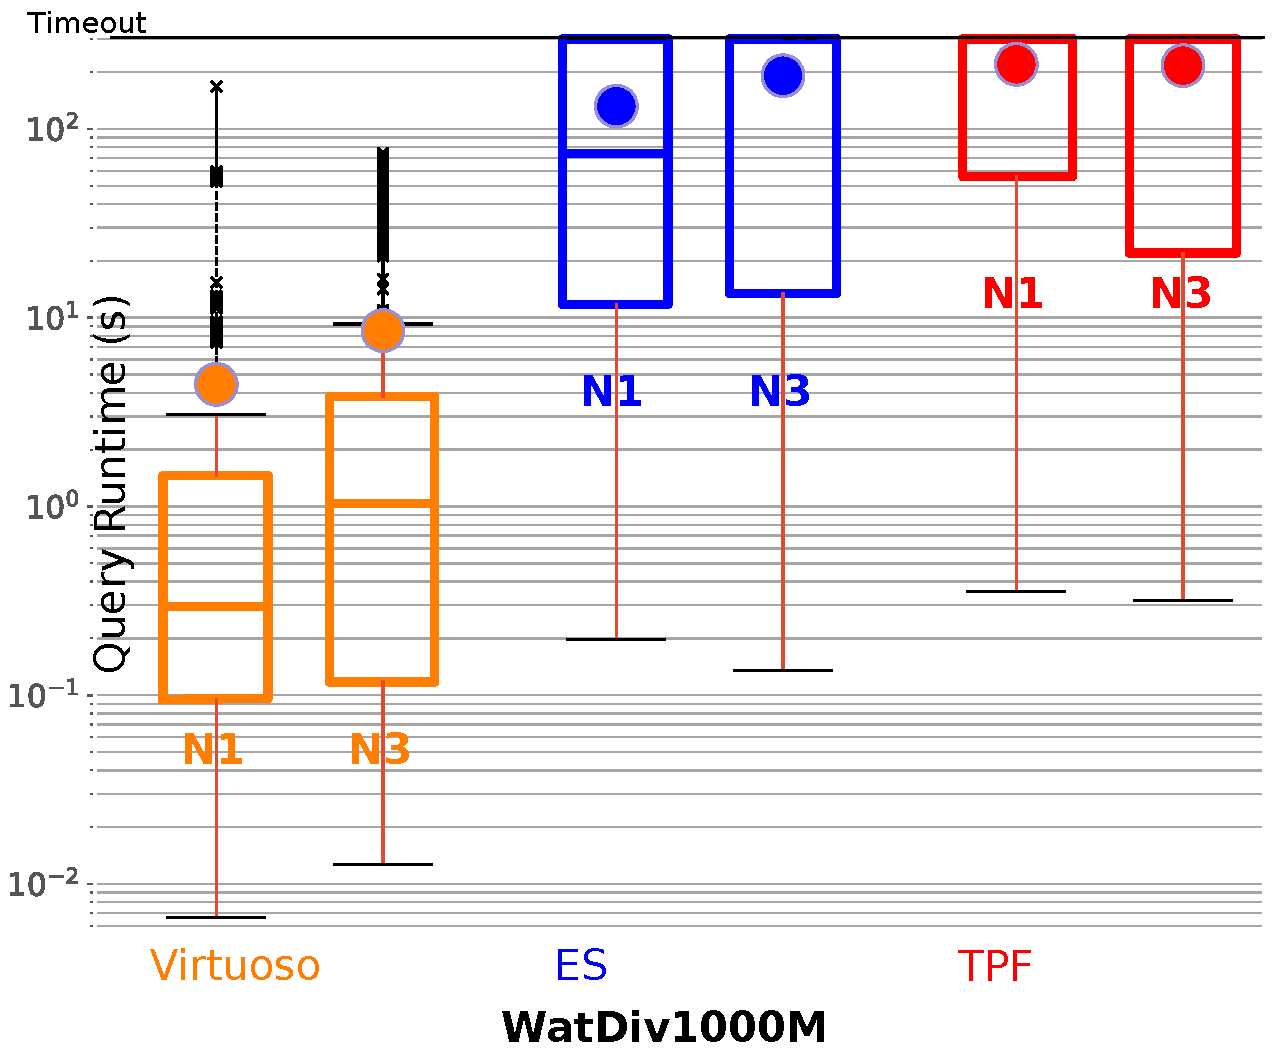
\includegraphics[width=0.9\linewidth]{imgs/Fig04_WatdivHorizontalScaling}
\caption{Pairwise comparison of query runtime distributions for single-node versus 3-node setups. None of the solutions achieve an average runtime speedup when adding more nodes, on the contrary overhead multipication factors of 1.9 and 1.5 are seen in left and center pane for \textbf{Vir3\_32\_Def} and \textbf{ES3\_32\_Def}. For \textbf{TPF3\_64\_Def} the overhead is negligible.}
\label{fig:Fig04_WatdivHorizontalScaling}
\end{figure}

\begin{figure*}[htbp!]
	\centering
	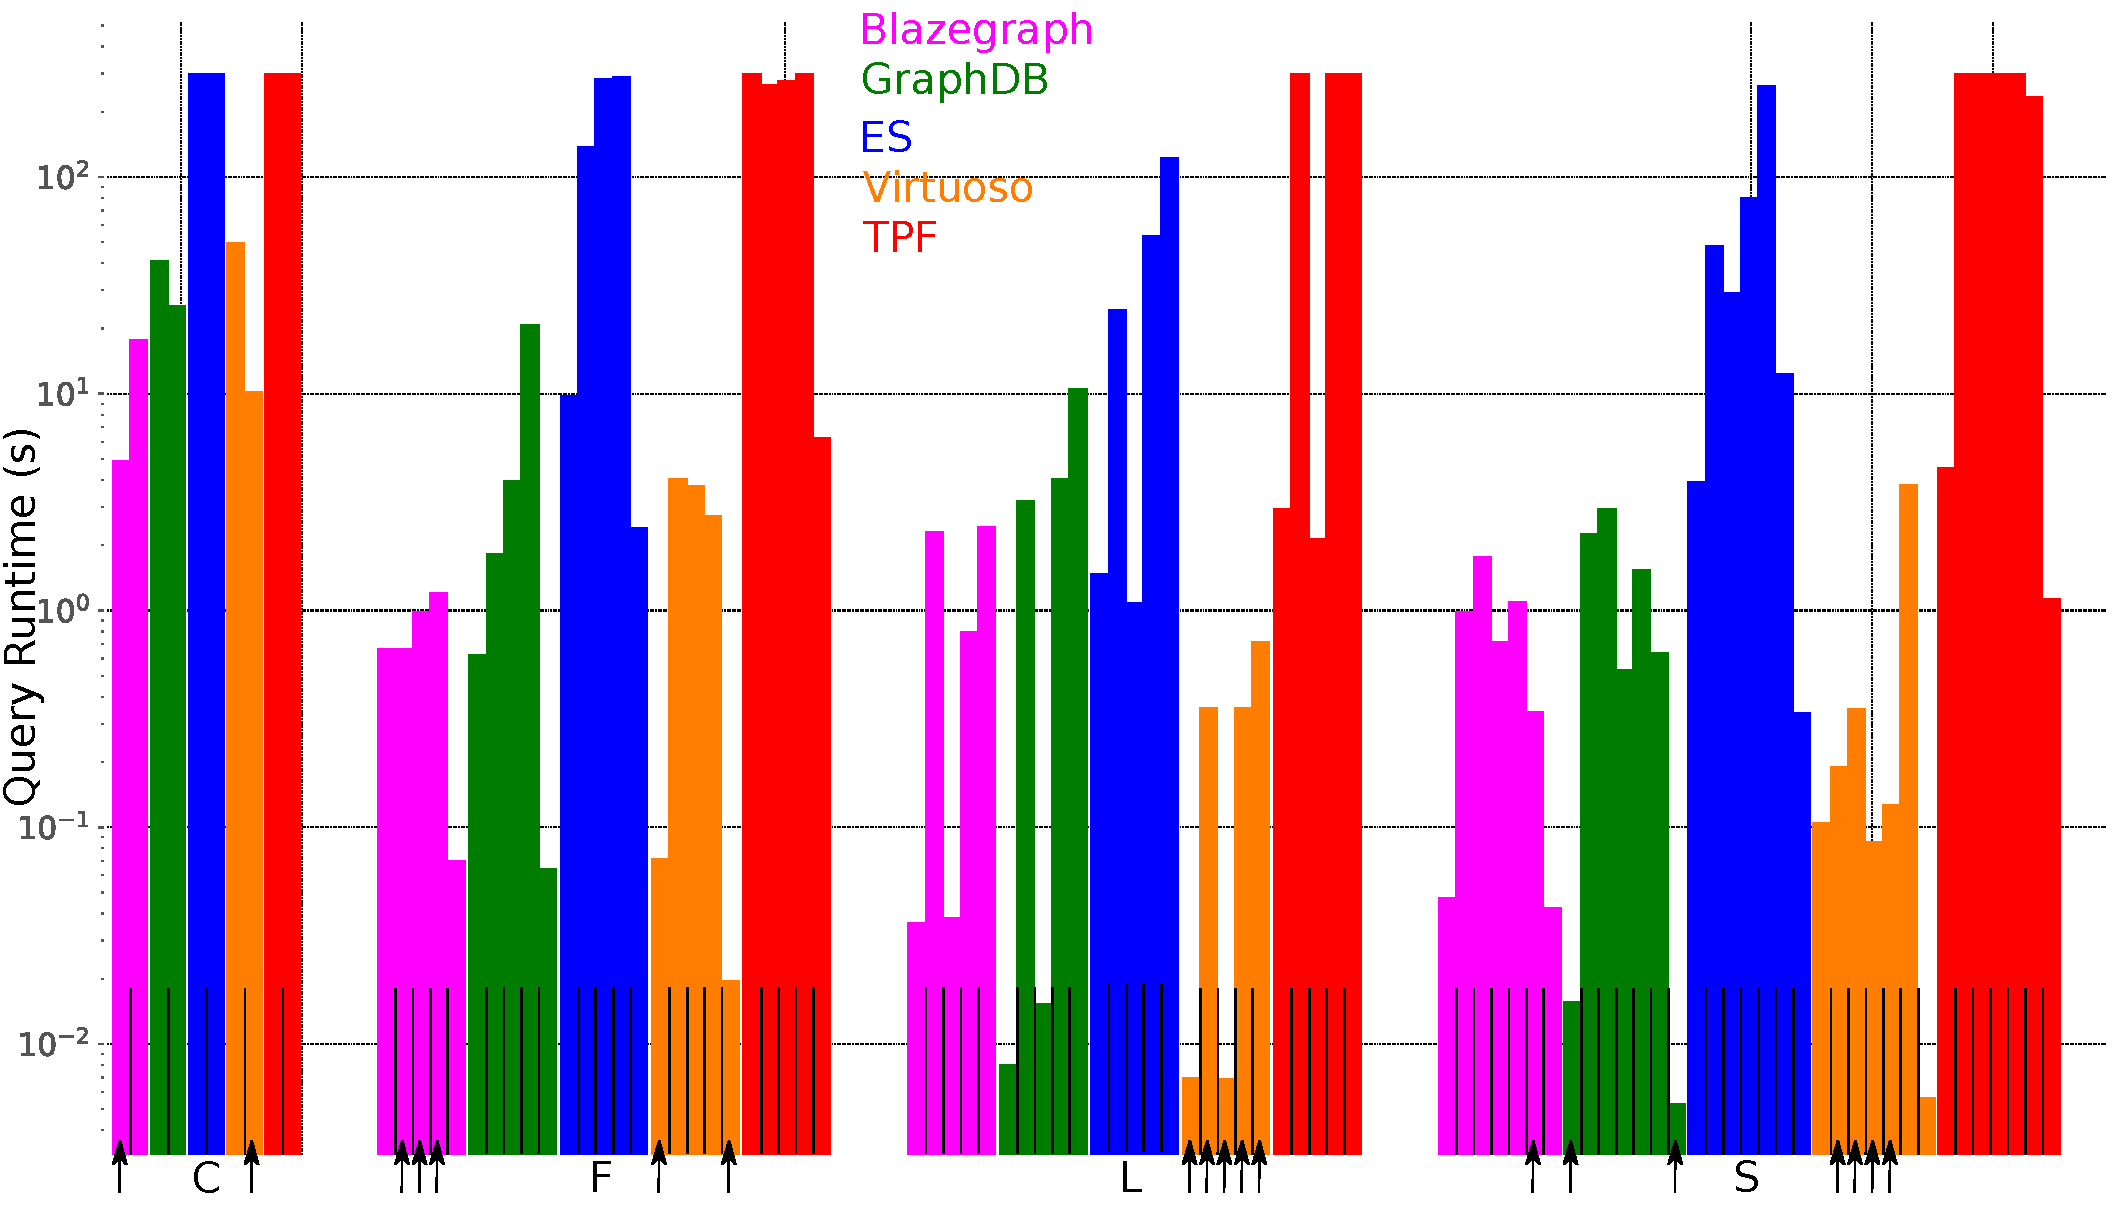
\includegraphics[width=0.9\linewidth]{imgs/Fig05_WatdivTemplates}
	\caption{Average Runtime per query template for 5 single-node setups. \textbf{TPF1\_64} has only 5 templates which do not coincide with the timeout of 300s, for \textbf{ES1\_64\_Def} this is alread 15 templates.
		\textbf{Vir1\_64\_Opt} is the fastest engine for 13 templates, \textbf{Gra1\_64\_Opt} for and \textbf{Bla1\_64\_Opt} for 3 templates each. Template \textbf{C3} was omitted due to query completeness issues. Blazegraph was the only engine to retrieve all results. } 
	\label{fig:Fig05_WatdivTemplates}
\end{figure*}

An alternative to increasing the memory in a single-node server is to increase the overall resources by 
adding more nodes, thus creating a distributed system. 

All 4 commercial RDF solutions support multi-node setups. GraphDB however, works only as a HA-solution (High-Availability): We did not evaluate this approach since 
it requires all data to be replicated on every node and does not support data partitioning, which is required to scale beyond the single-node resource limits.
The performance can however be estimated since it is equivalent to a setup with N identical databases with a load balancer equally distributing the queries between
the database replicas. The effect is a linear speedup in terms of completing a full query-mix. 
Virtuoso also supports a similar setup.
The effect on the indiviual query runtimes should be limited, but not
completely absent since the database load on the individual nodes will be smaller. The effect of database load on the query runtimes will be studied in the next section.


For Blazegraph support is required for setting up the multi-node system. This support was requested via the RFI but not fulfilled, which limited our comparison to \textbf{Vir3\_32\_Def}, \textbf{ES3\_32\_Def}, and \textbf{TPF3\_64\_Def}.

In Figure~\ref{fig:Fig04_WatdivHorizontalScaling} we show pairwise comparisons of the three setups for which we have both a single and a 3-node benchmark. 

\begin{itemize}
	\item \textbf{Benchmark survival interval:} %[('ES_N3_32_W1000_Def', 8684), ('Vir_N3_32_W1000_Def', 12000)]
	\textbf{Vir3\_32\_Def} and \textbf{TPF3\_64\_Def} managed to stay online during the entire Watdiv1000M benchmark, \textbf{ES3\_32\_Def} stopped responding after having completed 67\% of the multi-threaded run. 
	%Es_N3_32_W1000_Def:	Success: 34.8	Error: 65.1	Timeout: 0.0
	%Vir_N3_32_W1000_Def:	Success: 100.	Error: 0.0	Timeout: 0.0
	\item \textbf{Errors \& Timeouts:} 65\% of the queries of \textbf{ES3\_32\_Def} resulted in an HTTP 504 error, mentioning \textit{Gateway Timeout}. Further study revealed that this timeout was due to an internal configuration parameter in the ES distributed setup, unfortunately we did not receive any feedback on this issue. \textbf{Vir3\_32} successfully completed all queries. 70.6\% of the queries result in a timeout for \textbf{TPF3\_64\_Def}.
	\item \textbf{Multi-node overhead:} For all setups additional nodes lead to overhead instead of runtime speedup. Runtime multiplication factors are 1.9 and 1.5 for \textbf{Vir} and \textbf{ES}. \textbf{TPF} has a negligible overhead but is already very close to the query timeout.
\end{itemize}
%query_events_correct => double check on crash!
%Es: (Virtuoso 12k = all, TPF_64 also all)
% T1 warmup survival: 	2000
% T stress: 1343 - 1331 - 1348 - 1320 - 1348
%median/mean
%Vir_N1_32_W1000_Def    0.295139	4.431931
%Vir_N3_32_W1000_Def    1.040609	8.545433
%
%Es_N1_32_W1000_Def     74.091186 	132.011802
%Es_N3_32_W1000_Def    300.000000 	191.478380
%   
%LdF_N1_64_W1000_Def    300.0 		219.935204
%LdF_N3_64_W1000_Def    300.0		216.525390

In a discussion with OpenLink it was clarified that Virtuoso Cluster acts as a \emph{distributed memory solution}. This implies that adding nodes does not lead to a speedup in the query runtimes, but the total of memory pool in the system increases, allowing it to handle larger datasets for which a single node instance might not be suited. Since the single node benchmark did not exhaust the memory, there is no advantage to be expected from a multi-node setup. As an indication, according to support a 32GB machine should be able to manage up to 3 billion triples (10GB per 1B triples). 
This observation, together with the lack of feedback on the issues with \textbf{ES3\_32\_Def} and the high timeout percentage for \textbf{TPF3\_64\_Def} motivated our decision to not run any additional benchmarks with this approach for WatDiv1000M.

Systems translating SPARQL queries to distributed platforms such as Hadoop~\cite{cure2015evaluation, graux2016multi} are an alternative approach we did not test. 
Results for S2RDF~\cite{Schatzle:2016:SRQ:2977797.2977806} on Watdiv1000M indicate that a 10-node setup can be close to 10 times faster than a single-node Virtuoso server. Since these SPARQL-on-Hadoop solutions are not sufficiently mature and for example cannot be tested using a SPARQL endpoint definite conclusions can currently not be drawn. One observation to motivate this caution is the fact that Virtuoso is hardly affected when running multiple benchmark clients at once, as will be shown in section~\ref{subsec:load}. The operational cost for these Hadoop setups can also not immediately be deduced.